% 
% Annual Cognitive Science Conference
% Sample LaTeX Paper -- Proceedings Format
% 

% Original : Ashwin Ram (ashwin@cc.gatech.edu)       04/01/1994
% Modified : Johanna Moore (jmoore@cs.pitt.edu)      03/17/1995
% Modified : David Noelle (noelle@ucsd.edu)          03/15/1996
% Modified : Pat Langley (langley@cs.stanford.edu)   01/26/1997
% Latex2e corrections by Ramin Charles Nakisa        01/28/1997 
% Modified : Tina Eliassi-Rad (eliassi@cs.wisc.edu)  01/31/1998
% Modified : Trisha Yannuzzi (trisha@ircs.upenn.edu) 12/28/1999 (in process)
% Modified : Mary Ellen Foster (M.E.Foster@ed.ac.uk) 12/11/2000
% Modified : Ken Forbus                              01/23/2004
% Modified : Eli M. Silk (esilk@pitt.edu)            05/24/2005
% Modified: Niels Taatgen (taatgen@cmu.edu) 10/24/2006

%% Change ``a4paper'' in the following line to ``letterpaper'' if you are
%% producing a letter-format document.

\documentclass[10pt,letterpaper]{article}

\usepackage{cogsci}
\usepackage{pslatex}
\usepackage{apacite}
\usepackage{graphicx}
\usepackage{algorithmic}
\usepackage{amsmath}
\usepackage{amsfonts}
\usepackage{natbib}
\usepackage{algorithm2e}
\usepackage{sidecap}
\usepackage[figbotcap,tight,TABBOTCAP]{subfigure}

\usepackage{stmaryrd}
\newcommand{\sem}[1]{\ensuremath{\llbracket#1\rrbracket}}

\newcommand{\Gsep}{\mathbb{G}_{\text{sep}}}

\title{Learning to Reason Pragmatically with Cognitive Limitations}
 
\newcommand{\email}[1]{\texttt{#1}}

\author{
  {\large\textbf{Adam Vogel}}\\ 
  \email{acvogel@stanford.edu}\\
  Stanford Computer Science\\
  %Department of Computer Science\\
  %Stanford University
  \And 
  {\large\textbf{Andr{\'e}s Gom{\'e}z Emilsson}}\\
  \email{nc07agom@stanford.edu}\\
  Stanford Psychology
  %Department of Psychology\\
  % Stanford University
  \And 
  {\large\textbf{Michael C.~Frank}}\\
  \email{mcfrank@stanford.edu}\\
  Stanford Psychology\\
  %Department of Psychology\\
  %Stanford University
  \AND
  {\large\textbf{Dan Jurafsky}}\\
  \email{jurafsky@stanford.edu}\\
  Stanford Linguistics\\
  %Department of Linguistics\\
  %Stanford University
  \And
  {\large\textbf{Christopher Potts}}\\
  \email{cgpotts@stanford.edu}\\
  Stanford Linguistics\\
  %Department of Linguistics\\
  %Stanford University
}

\begin{document}

\maketitle


\begin{abstract}
Recursive Bayesian models of linguistic communication capture a
variety of intricate kinds of pragmatic enrichment, but they tend to
depend on the unrealistic assumption that agents are invariably
optimal reasoners. We present a discriminative model that seeks to
capitalize on the insights of such approaches while addressing these
concerns about inferential power. The model relies on only approximate
representations of language and context, and its recursive properties
are limited to the training phase. The resulting behavior is often not
optimal, but we present experimental evidence that this suboptimal
behavior is closely aligned with human performance on both simple and
complex reference games.


%\textbf{Keywords:} 
%Add your choice of indexing terms or keywords; kindly use a semi-colon; between each term.
\end{abstract}

\section{Introduction}\label{sec:intro}
Recursive Bayesian models of language production and comprehension
capture a variety of intricate phenomena concerning context dependence 
and pragmatic enrichment 
\citep{Jaeger:2007,
Franke09DISS,
Frank:Goodman:2012,
Bergen:Goodman:Levy:2012,
Vogel-etal:2013,
Smith:Goodman:Frank:2013}.
In these models, speakers and listeners reason about each other
recursively in order to achieve ever more optimal communication
systems. These approaches offer precise, algorithmic perspectives on
philosophical and linguistic theories of communication
\citep{Lewis69,Grice75,Horn84}, and they make robust predictions about
experimental data
\citep{Stiller:Goodman:Frank:2011,Rohde-etal:2012,Degen-etal:2013}.

Despite the success of these models, they raise concerns about
inferential power, in that they assume that the agents are
invariably optimal reasoners with unbounded computational resources.
These concerns can be mitigated by stipulations about depth of
iteration \citep{CamererHo:2004,Franke09DISS,Jaeger:2007,Jaeger:2011}, but the
models remain computationally demanding and powerful.

We seek to capitalize on the insights of these approaches while
addressing these concerns. We define a discriminative model of
pragmatic reasoning that requires no explicit representation of the
context. Rather, it relies only on features of the environment and
language. In addition, the recursive aspects of the model are limited
to training: we employ a \emph{self-training} regime in which,
starting with basic models of the speaker and the hearer, we use the
speaker to generate supervised training data for the listener, and
vice versa. Once this phase is complete, the model makes decisions
without any recursion. The models are both more efficient and more
fallible than the above generative ones. 

Our model also offers a way to reconcile previous explanations of the
interpretation or production of pragmatically complex utterances:
slowly via complex recursive inferences made as each sentence is
processed, \citep{Geurts09,Huang:Snedeker:2009} or quickly via
inferences that are pre-compiled and cached based on previous
interactions
\citep{Levinson00,Grodner-etal:2010,Smith:Goodman:Frank:2013}. Instead,
our discriminatively-trained model instantiates a third possibility,
extending \citealt{Jurafsky04}: learning to directly map surface
linguistic cues to speaker intent. Like the interpretive models, a
learned model explains how context-sensitive inferences could be drawn
at communication time; like the cached models, it explains why
processing could be fast and direct.

Our central question is whether our model's behavior matches human
performance across a wide range of situations. To address this, we use
collaborative reference games
\citep{Rosenberg:Cohen:1964,Clark:Wilkes-Gibbs:1986,DeVault-etal:2005}
in which a speaker refers to an object in a shared visual scene and
the listener uses the speaker's message to try to guess the intended
referent. By manipulating the properties of the scene and the
speaker's available messages, we can ensure that pragmatic reasoning,
of various levels of complexity, is required for reliable success. We
report several experiments that seek to identify the bounds on human
performance in these reference games, and we compare human performance
to our model, showing that its inferences closely align with human
performance.



\section{Reference Games}\label{sec:refgames}
Figure~\ref{fig:scalesStimulus} depicts a reference game
scenario. There are three potential referents (A, B, and C), each with
a pre-specified set of properties (wearing glasses, wearing a hat,
having a mustache). The \emph{speaker} is privately assigned one of
the referents. Using a message from a pre-defined vocabulary, the
speaker tries to convey the identity of this referent to the
\emph{listener}. The listener uses the message to choose one of the
referents. Intuitively, the two participants' goals are aligned: they
win just in case the speaker's referent is the hearer's choice.

\begin{figure}[ht]
  \centering
  % 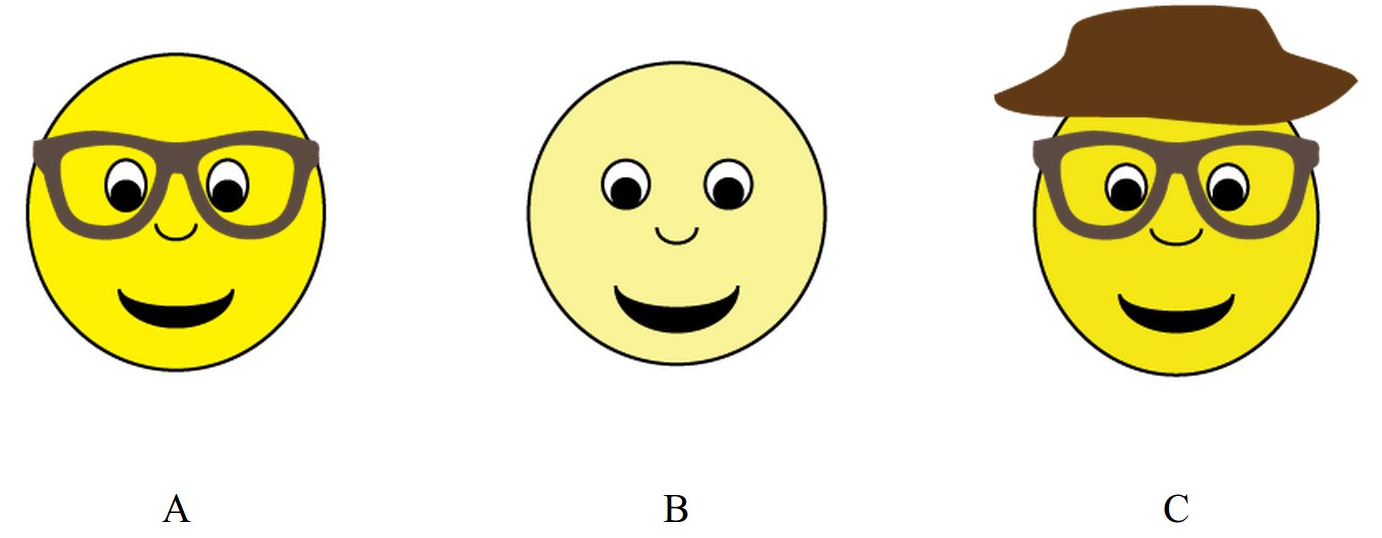
\includegraphics[width=\columnwidth]{fig/facesScales.png}
  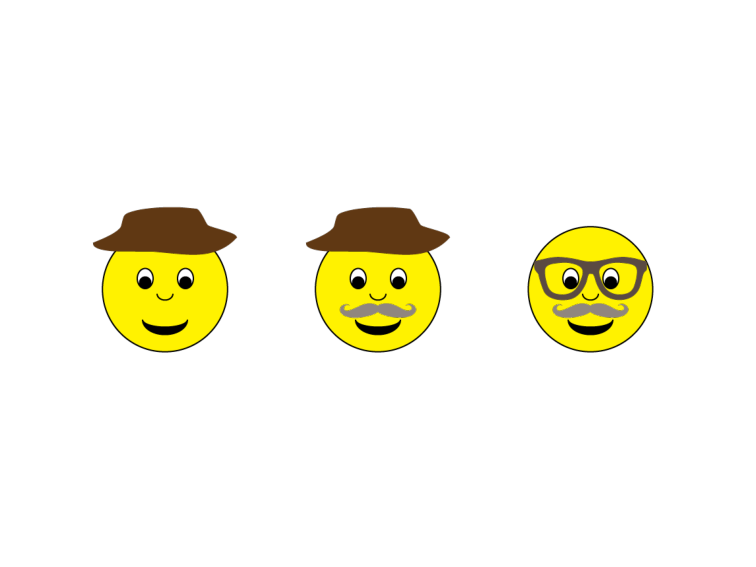
\includegraphics[width=0.7\columnwidth]{fig/refgame-sample}

  \vspace{-4pt}
  
  A\hspace{55pt}B\hspace{55pt}C
  \caption{Scenario for a simple reference game.}
  \label{fig:scalesStimulus}
\end{figure}

\subsection{Definition}
Formally, a reference game is a tuple $G = (M,T,\sem{\cdot})$, where
$T$ is the set of targets, $M$ is the set of messages, and
$\sem{\cdot} : M \to 2^{T}$ is the semantics of the messages, which
dictates which targets each message is true of.  A speaker $S$ is a
(possibly stochastic) function $G \times T \to M$ from a game and
target to a message. Similarly, a listener $L$ is a function $G \times
M \to T$ from a game and a message to a target.  For a given run of a
game $G$ and target $t$, the speaker produces the message $m =
S(G,t)$, the listener selects a target $t' = L(G,m)$, and they win iff
$t = t'$.

\subsection{Literal Speaker and Listener}
To initialize the learning procedure described in the next section, we
define literal speakers and listeners, who rely entirely on the
semantics of the messages, with no consideration of the other
participant's behavior. The literal speaker $S_{0}$, when given a
target to refer to, picks uniformly at random from messages which are
true of the target:
%
\begin{equation}
S_{0}(G,t)  = \text{Uniform}\left(\{m \vert t \in \sem{m}\}\right)
\end{equation}
%
Similarly, the literal listener $L_0$, when given a message $m$, picks
randomly from targets in the semantics of the message:
%
\begin{equation}
L_{0}(G,m) = \text{Uniform}\left(\{t \vert t \in \sem{m}\}\right)
\end{equation}



\section{Discriminative Best Response}\label{sec:model}
Our model relies on iterated \emph{self-training}, alternating
between discriminatively training the listener and the speaker.  This
method requires no generative model of the context or messages, but
rather only a shallow feature vector representation.  Furthermore,
there is no explicit recursive reasoning procedure of the sort common
in the generative approaches discussed above.  At evaluation time, our
trained listener simply generates features for the problem and
utterance, and computes the model activation for each possible target.

Algorithm~\ref{alg:selftrain} describes the training algorithm. It
takes as input a set of reference games $\mathbb{G}$, and a number of
training iterations to perform, $N$.  Starting with the literal
speaker, we train a listener using the input reference games and the
speaker (Algorithm~\ref{alg:train-listener}). Then, using this newly
trained listener, we retrain the speaker
(Algorithm~\ref{alg:train-speaker}), using the current listener to
create training data.  We use an artificial neural network (ANN) as
the discriminative classifier, but other learning algorithms would
work as well.  This procedure repeats for $N$ iterations, yielding a
self-trained ANN listener and speaker.

To train a listener (Algorithm~\ref{alg:train-listener}), we use a
speaker $S$ to generate training data as follows.  For each reference
game $G \in \mathbb{G}$, and for each target $t \in T$, we query the
speaker to get the speaker's chosen message $m = S(G,t)$.  We then
form a training set in which the input features are games combined
with messages and the gold label is the target $t$ that the speaker
intended to refer to. The listener ANN uses a simple feature
representation: a binary feature for the presence or absence of each
feature for each target, and also a binary feature for each possible
message. For three targets, three properties, and three utterances,
this yields twelve binary features. The listener ANN has three
outputs, one per target. Given a reference game and a message, the
listener selects the target corresponding to the highest output
activation.

The training procedure for speakers
(Algorithm~\ref{alg:train-speaker}) proceeds similarly. For each
reference game $G \in \mathbb{G}$ and for each target $t \in T$, we
query the listener to determine whether there is a message $m$ that
the listener interprets as target $t$.  If so, we add a training
example with $(G, t)$ as the features and $m$ as the label.  For some
listeners, there is no message it interprets as a particular target,
so we do not add those to the training set.

The listener and speaker ANNs have the same structure: a
fully-connected network with 12 input features, one a hidden layer 
whose size we vary in the experiments, and 3 output nodes. The models 
are trained with back propagation \citep{Rumelhart-etal:1986}, using 
the PyBrain library \citep{Schaul:2010:PYB:1756006.1756030}.


\begin{algorithm}
{\bf Algorithm: }SelfTrain\\
\KwIn {Reference games $\mathbb{G}$, Number of iterations $N$}
\KwOut{Listener $L$}
Initialize $S = S_0$\\
\For {i from $1$ to $N$} {
$L = TrainListener(\mathbb{G}, S)$\\
$S = TrainSpeaker(\mathbb{G}, L)$\\
}
\Return {$L$}\\
~\\
\caption{Train listener and speaker ANNs for a given number of iterations, starting from the literal speaker $S_0$.}
\label{alg:selftrain}
\end{algorithm}

\vspace{-12pt}

\begin{algorithm}
{\bf Algorithm: }TrainListener\\
\KwIn {Reference games $\mathbb{G}$, Speaker $S$}
\KwOut{Listener $L$}
Initialize training data $X = Y = \emptyset$\\
\ForEach{Reference game $G = (T,M) \in \mathbb{G}$} {
  \ForEach{Target $t \in T$} {
    $m = S(G,t)$\\
    Append $(G,m)$ to $X$\\
    Append $t$ to $Y$\\
  }
}
\Return{$\text{ANN-Train}(X,Y)$}\\
~\\
\caption{Train a listener ANN from a given speaker.}
\label{alg:train-listener}
\end{algorithm}

\begin{algorithm}
{\bf Algorithm:} TrainSpeaker\\
\KwIn {
  Reference games $\mathbb{G}$, Listener $L$
}
\KwOut{Speaker $S$}
Initialize training data $X = Y = \emptyset$\\
\ForEach{Reference game $G = (T,M) \in \mathbb{G}$} {
  \ForEach{Target $t \in T$} {
    \If {$\exists m$ such that $L(G,m) = t$} {
      Append $(G,t)$ to $X$\\
      Append $m$ to $Y$\\
    }
  }
}
\Return {$\text{ANN-Train}(X,Y)$}\\
~\\
\caption{Train a speaker ANN from a given listener.}
\label{alg:train-speaker}
\end{algorithm}



\section{Simulations with Synthetic Data}
We first evaluate our ANN listener model on a variety of automatically
generated reference games.

\subsection{Experimental Design}

We first generated the full set $\Gsep$ of three-target, three-feature
reference games that have fully separating equilibria, that is, games
that can be resolved to totally unambiguous speaker and listener
strategies in the iterated best response (IBR) model of
\citet{Franke09DISS} and \citet{Jaeger:2007,Jaeger:2011}. From
$\Gsep$, we generated 1,206 specific reference instances, where an
instance is a game $G$, a message $m$, and an intended target $t$. We
separate these instances by the depth of reasoning that an IBR
listener requires to identify a unique target. Using these instances
$(G, m, t)$, we self-train our listener model using only the game
information $G$ and the message $m$, holding out the target $t$ for
evaluation, as described in Algorithm~\ref{alg:selftrain}.

\subsection{Results}

We first evaluated how the number of training iterations affects model
performance. Figure~\ref{fig:synthetic} shows how the accuracy of the
training model changes over training iterations. The x-axis is how
many training iterations the listener underwent. (The listener with 0
training iterations is the literal listener.) The y-axis is the
precision of the model on the specific type of problem. We next
explored how the size of the hidden layer affects listener
performance, by varying the size of the hidden layer and evaluating
each model's performance after 10 training iterations
(Figure~\ref{fig:syntheticHidden}).


%\begin{figure}
%    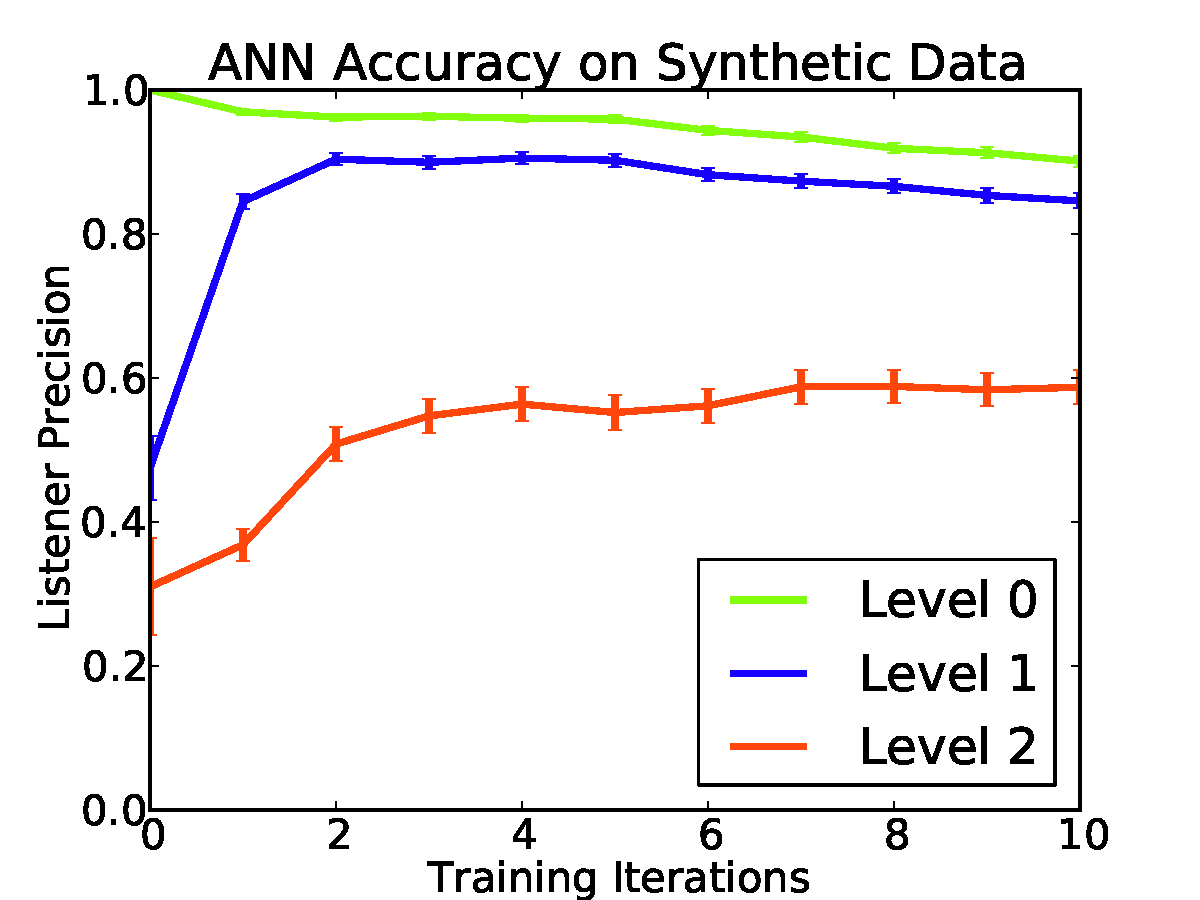
\includegraphics[width=\columnwidth]{fig/synthetic.pdf}
%    \caption {Listener accuracy on synthetic problems by number of training iterations, for a model with 50 hidden nodes.}
%    \label{fig:synthetic}
%\end{figure}
%
%\begin{figure}
%  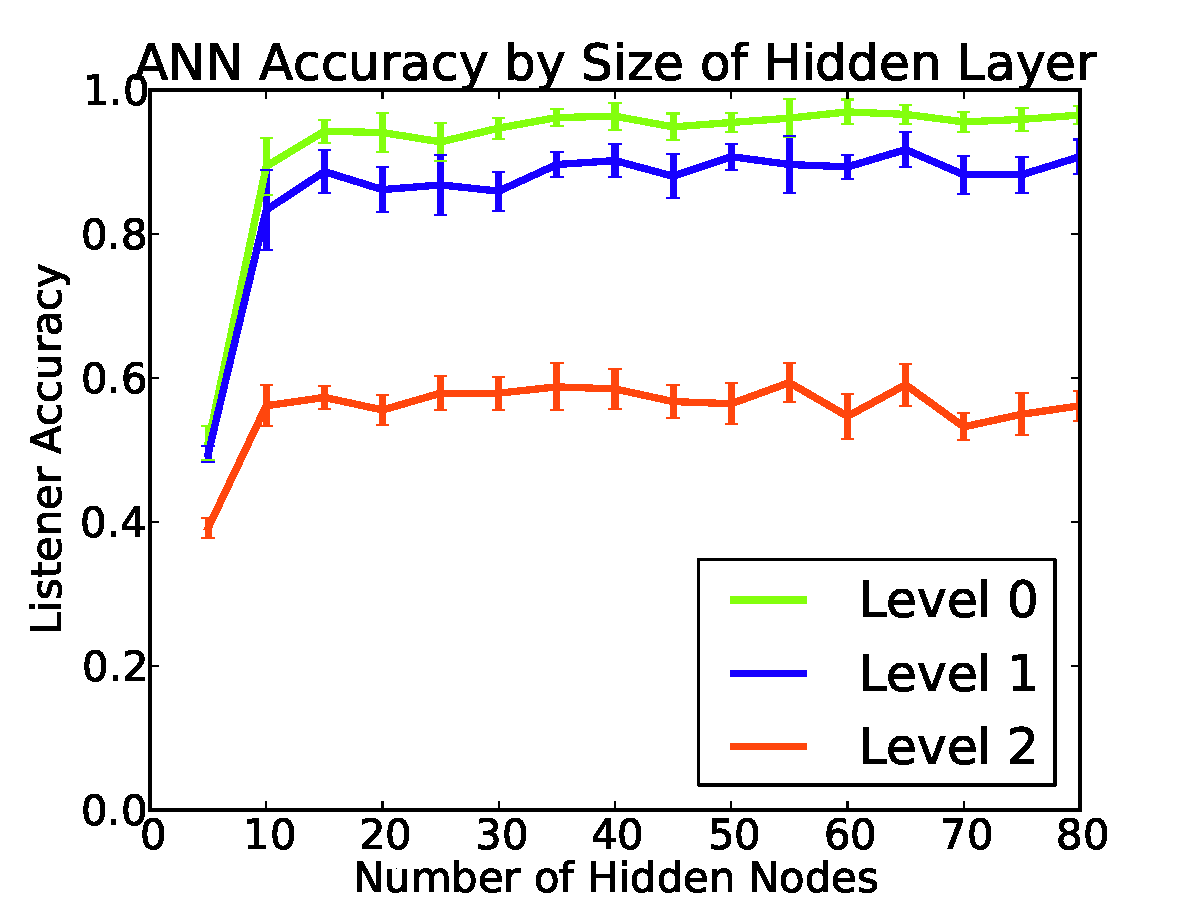
\includegraphics[width=\columnwidth]{fig/hiddenSynthetic.pdf}
%  \caption {Listener accuracy on synthetic problems while varying the size of the hidden layer.}
%  \label{fig:syntheticHidden}
%\end{figure}

\subsection{Discussion}

Model accuracy decreases as the problem level (complexity) increases.
The literal speaker performs perfectly on level~0 problems, as
expected. It is surprising that the trained models perform less than
perfectly on these easy problems. A listener trained \emph{only} on
level 0 problems achieves perfect accuracy on level~0 problems, so it
seems that training on the more difficult problems leads to some
degradation in performance on easy problems. The trained listeners
perform well, with 91\% accuracy on level~0, 85\% on level~1 problems,
and 59\% on level~2 problems.
Figure~\ref{fig:syntheticHidden} shows that the size of the hidden layer 
has some effect on model performance, but that after a certain threshold 
the performance stabilizes.

We also evaluated IBR listener models for a variety of recursion 
depths (Figure~\ref{fig:syntheticIBR}). All have perfect accuracy on
the level 0 problems (barely visible along the top of the plot), with
rapidly increasing accuracy on the level 1 and 2 problems. The
accuracies shown here are using the probabilities of each target given
a message \citep{Frank:Goodman:2012,Bergen:Goodman:Levy:2012}. If we
instead always choose the target with the highest probability given a
message \citep{Franke09DISS,Jaeger:2007,Jaeger:2011}, the IBR model
solves the problems exactly after one and two levels, respectively.

\begin{figure}[ht]
  \centering
  \subfigure[Varying the number of training iterations, with 50 hidden nodes.]{
    \parbox[c]{\columnwidth}{
      \centering
      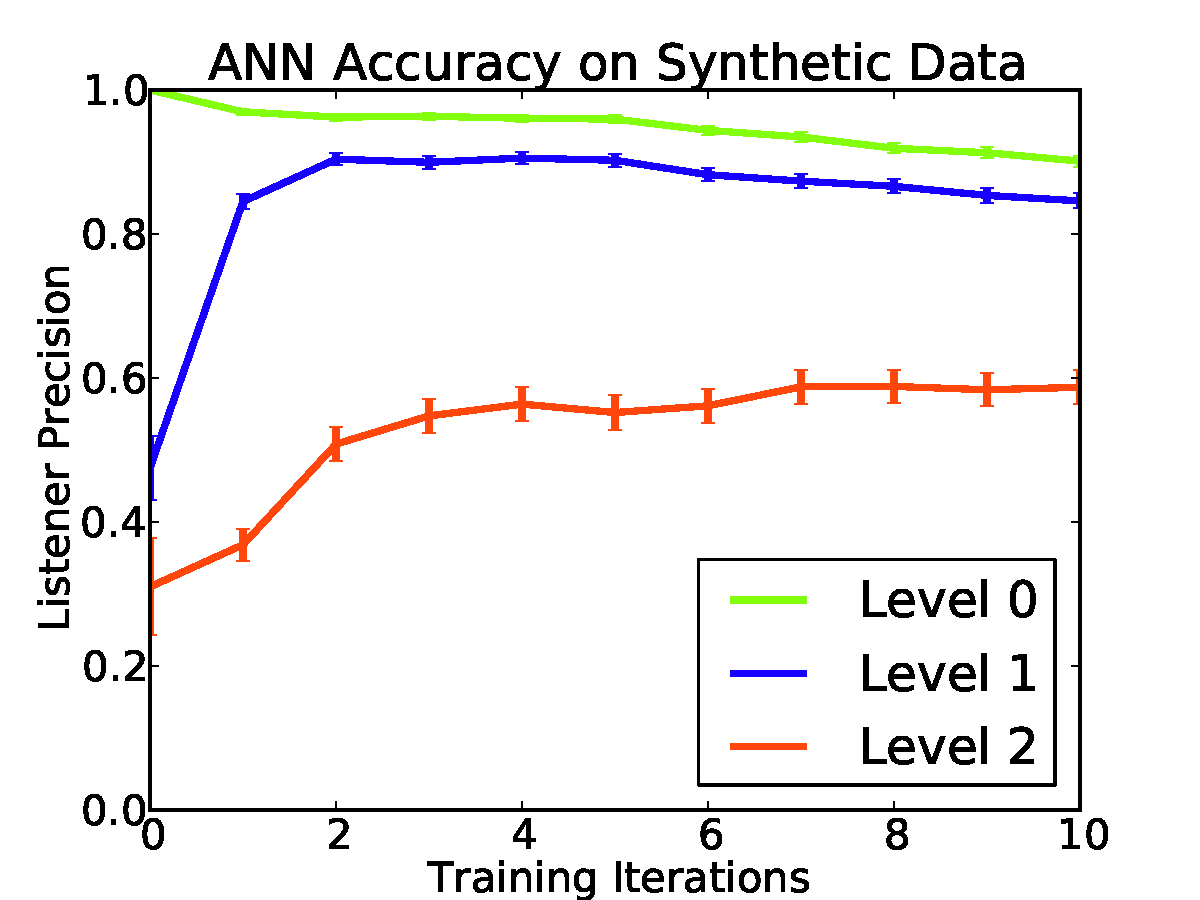
\includegraphics[width=0.8\columnwidth]{fig/synthetic.pdf}
    }
    \label{fig:synthetic}
  }

  \vspace{-2mm}

  \subfigure[Varying the number of hidden nodes, for 10 training iterations.]{    
    \parbox[c]{\columnwidth}{
      \centering
      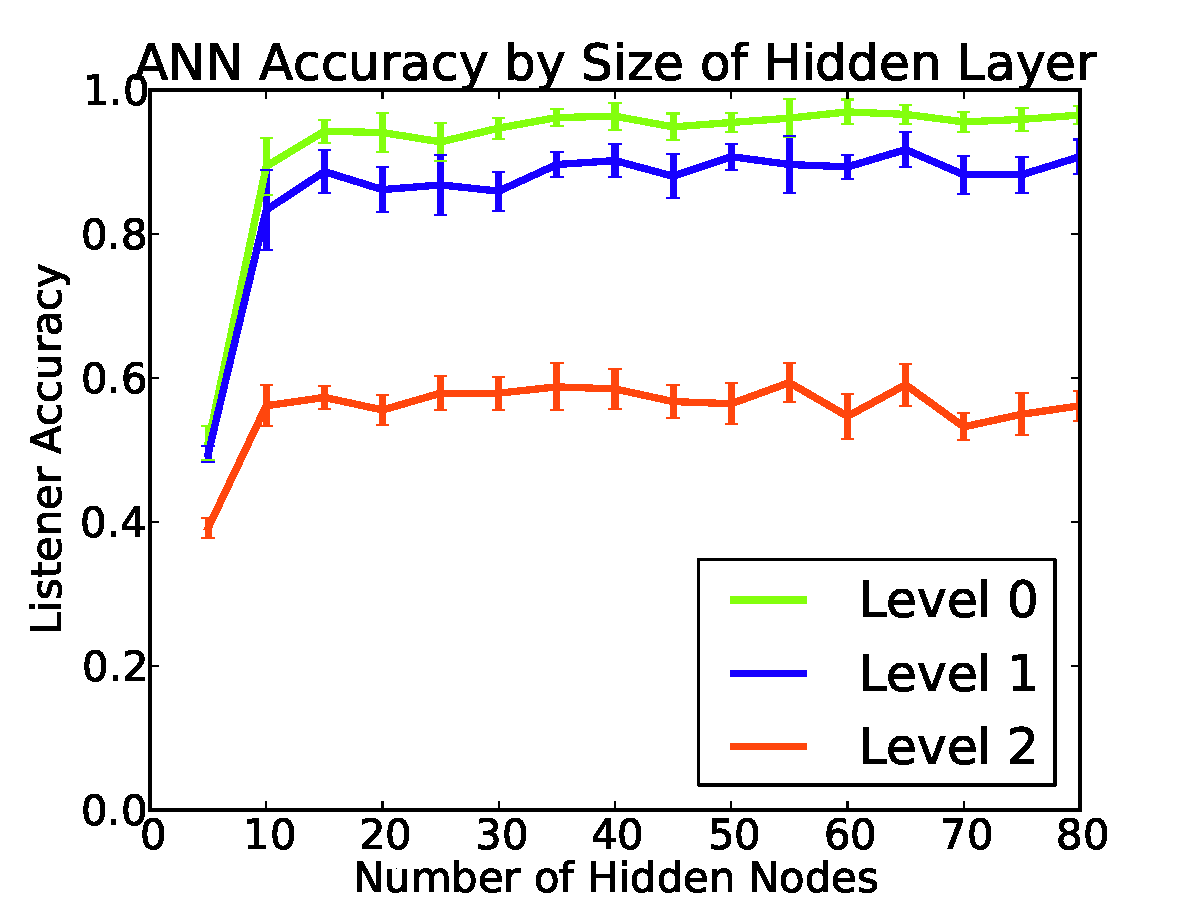
\includegraphics[width=0.8\columnwidth]{fig/hiddenSynthetic.pdf}
    }
    \label{fig:syntheticHidden}
  }
  \vspace{-4mm}
  \caption{ANN Listener accuracy on synthetic data.}
\end{figure}

\begin{figure}[ht]
  \centering
  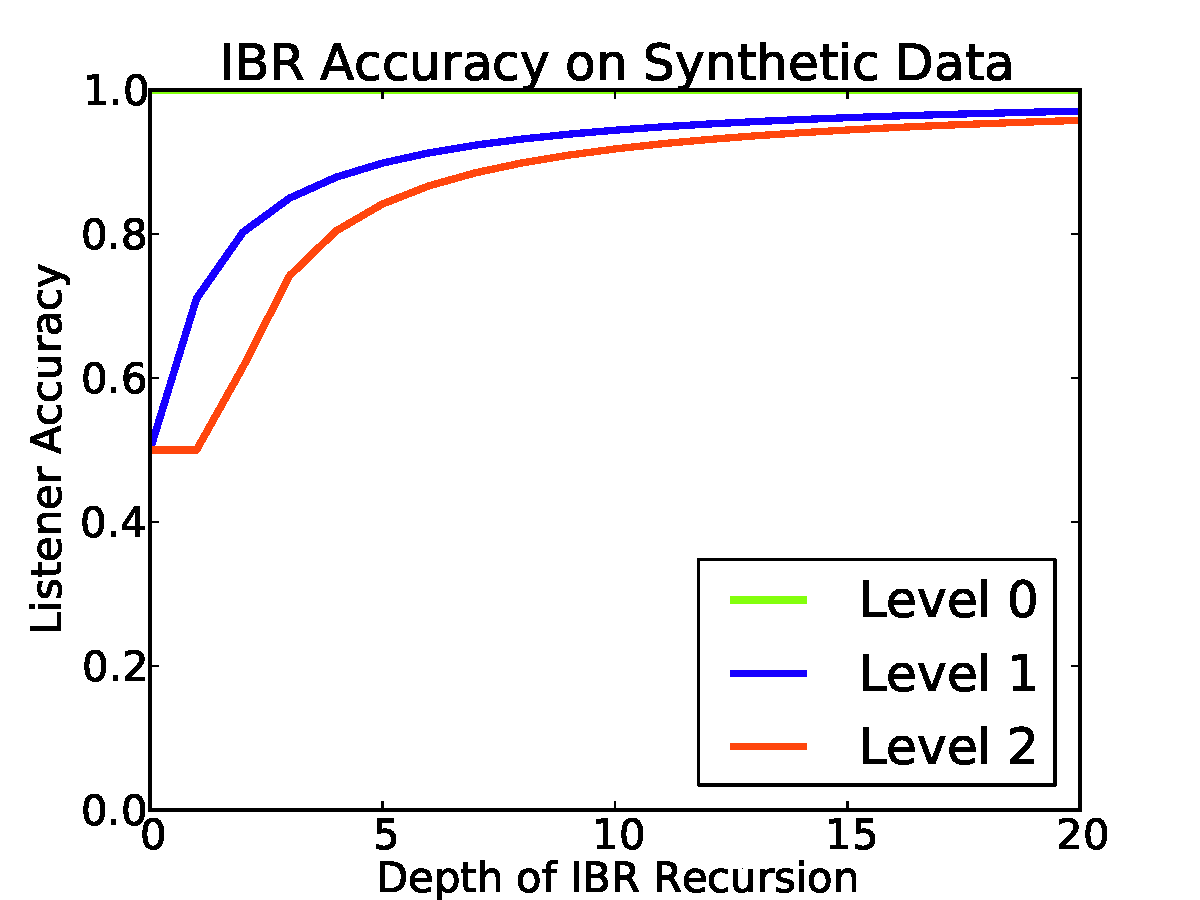
\includegraphics[width=0.8\columnwidth]{fig/IBRsynthetic.pdf}
  \vspace{-4mm}
  \caption{IBR listener accuracy on synthetic problems.}
  \label{fig:syntheticIBR}
\end{figure}


% \section{Human Subject Experiments}
\begin{figure*}
% [htp]
  \centering
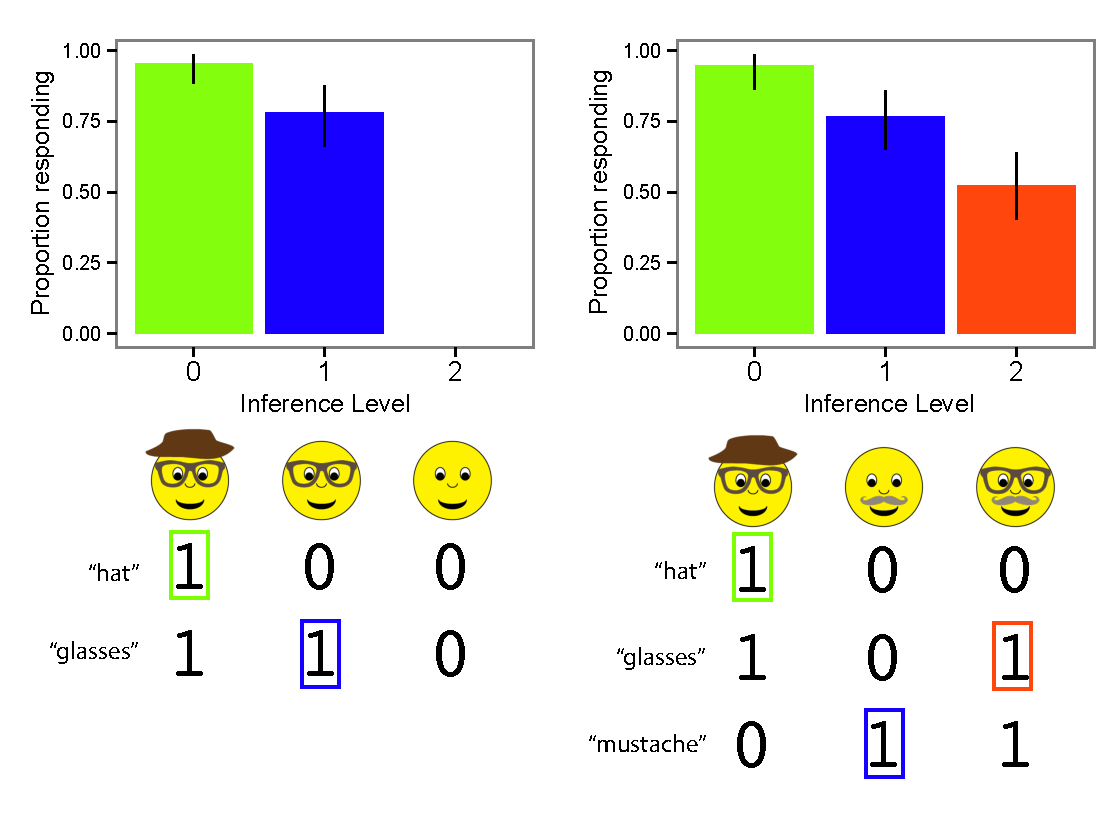
\includegraphics[width=4.75in]{fig/ann-ibr-bargraph.pdf}
\caption{\label{fig:humans} Human data and experimental matrices from Experiments 1 and 2.}
\end{figure*}

\begin{figure*}[t]
  \centering
  \subfigure[ANN Simple]{
    \centering
    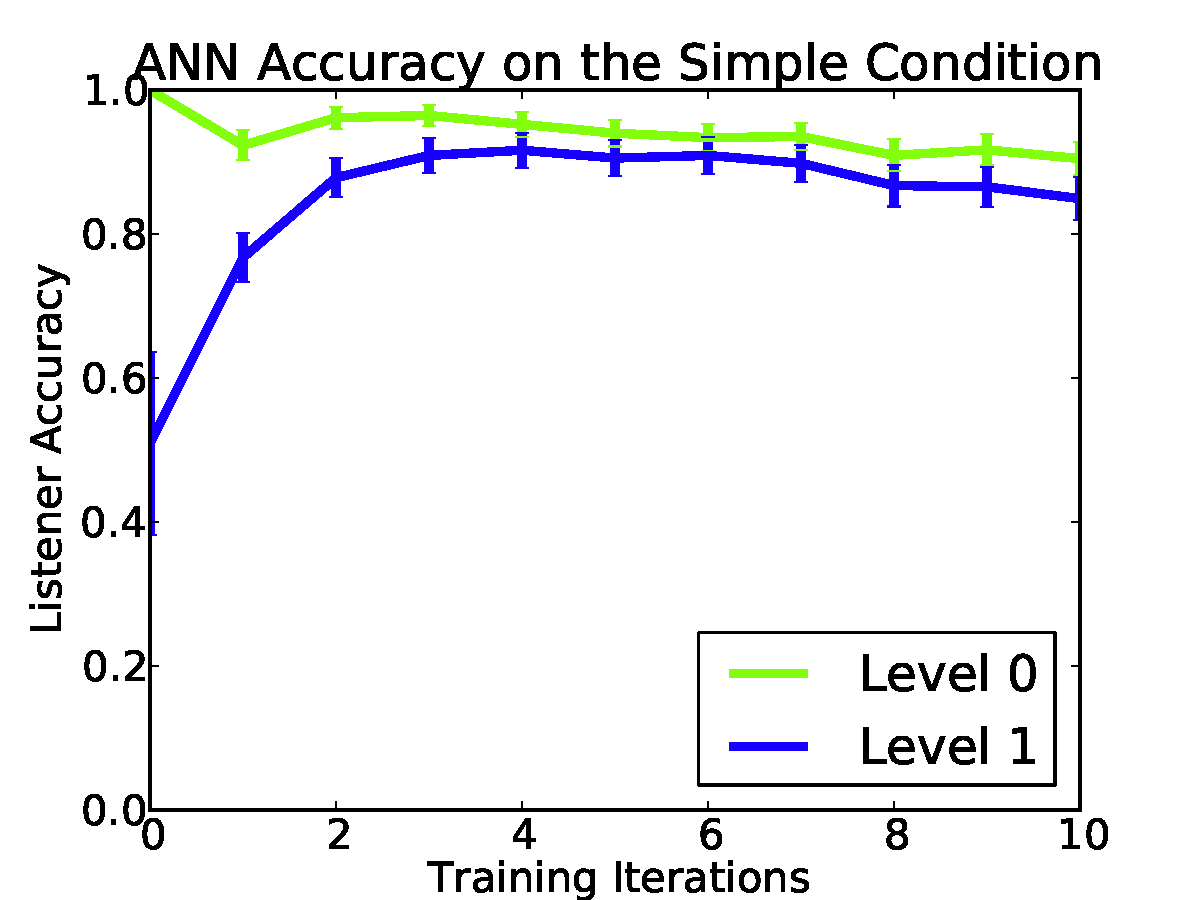
\includegraphics[width=0.8\columnwidth]{fig/scales.pdf}
    \label{fig:scales}
  } 
  \hspace{40pt}
  \subfigure[ANN Complex]{
    \centering
    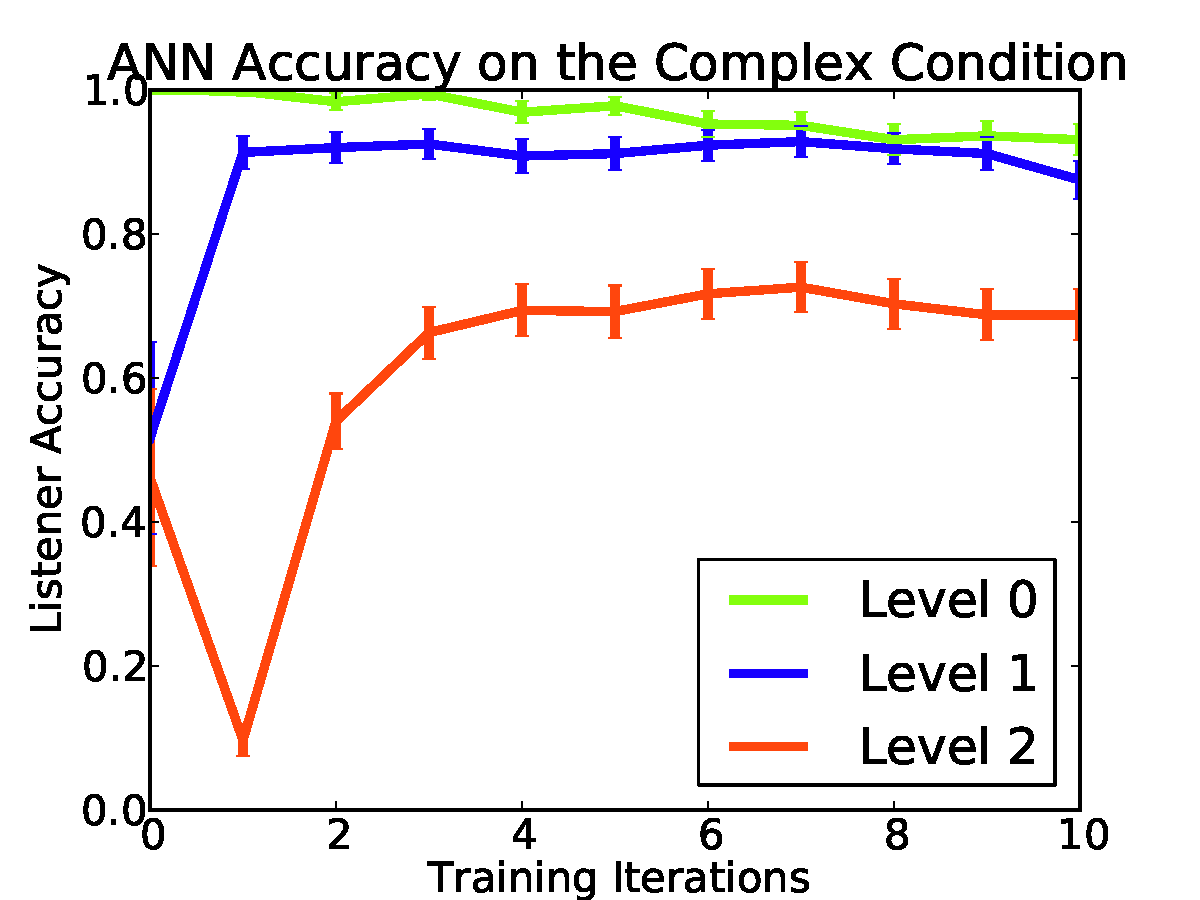
\includegraphics[width=0.8\columnwidth]{fig/scalesPlus.pdf}
    \label{fig:scalesPlus}
  }
  \caption{Evaluation of the ANN listener with 50 hidden nodes on the simple (a) and complex (b) settings.}

  \subfigure[IBR Simple]{
    \centering
    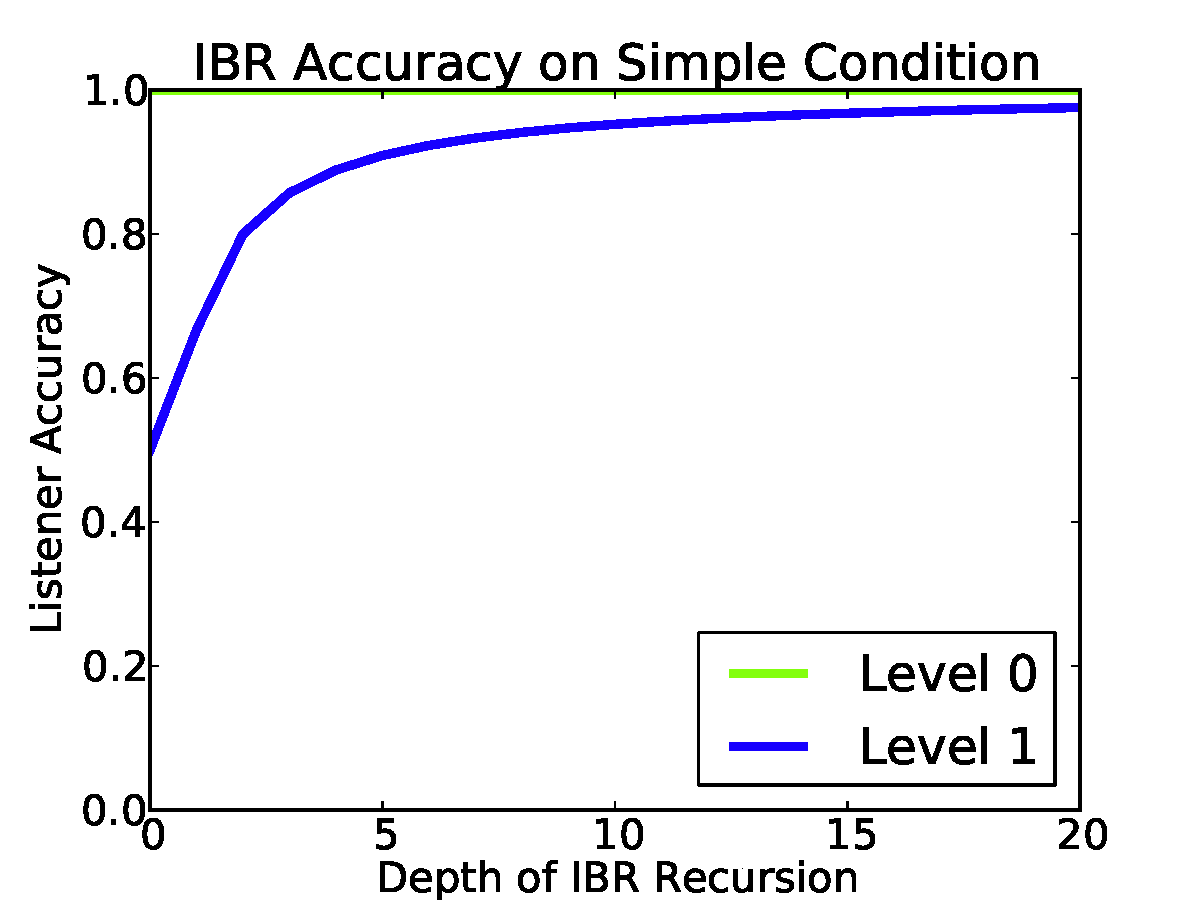
\includegraphics[width=0.8\columnwidth]{fig/IBRscales.pdf}
    \label{fig:ibrScales}
  } 
  \hspace{40pt}
  \subfigure[IBR Complex]{
    \centering
    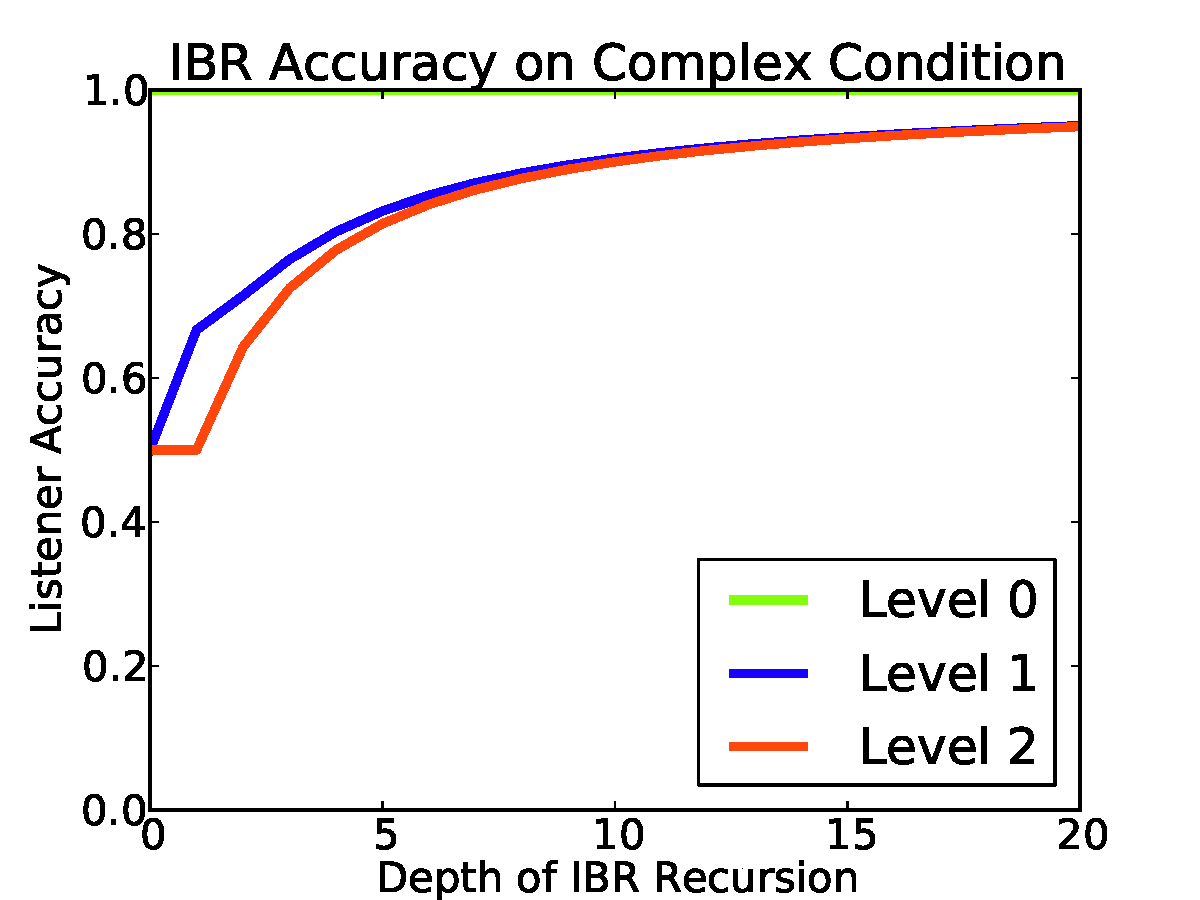
\includegraphics[width=0.8\columnwidth]{fig/IBRscalesPlus.pdf}
    \label{fig:ibrScalesPlus}
  }
  \caption{Evaluation of IBR listeners with different depths of recursion.}
\end{figure*}


%\begin{figure}
%    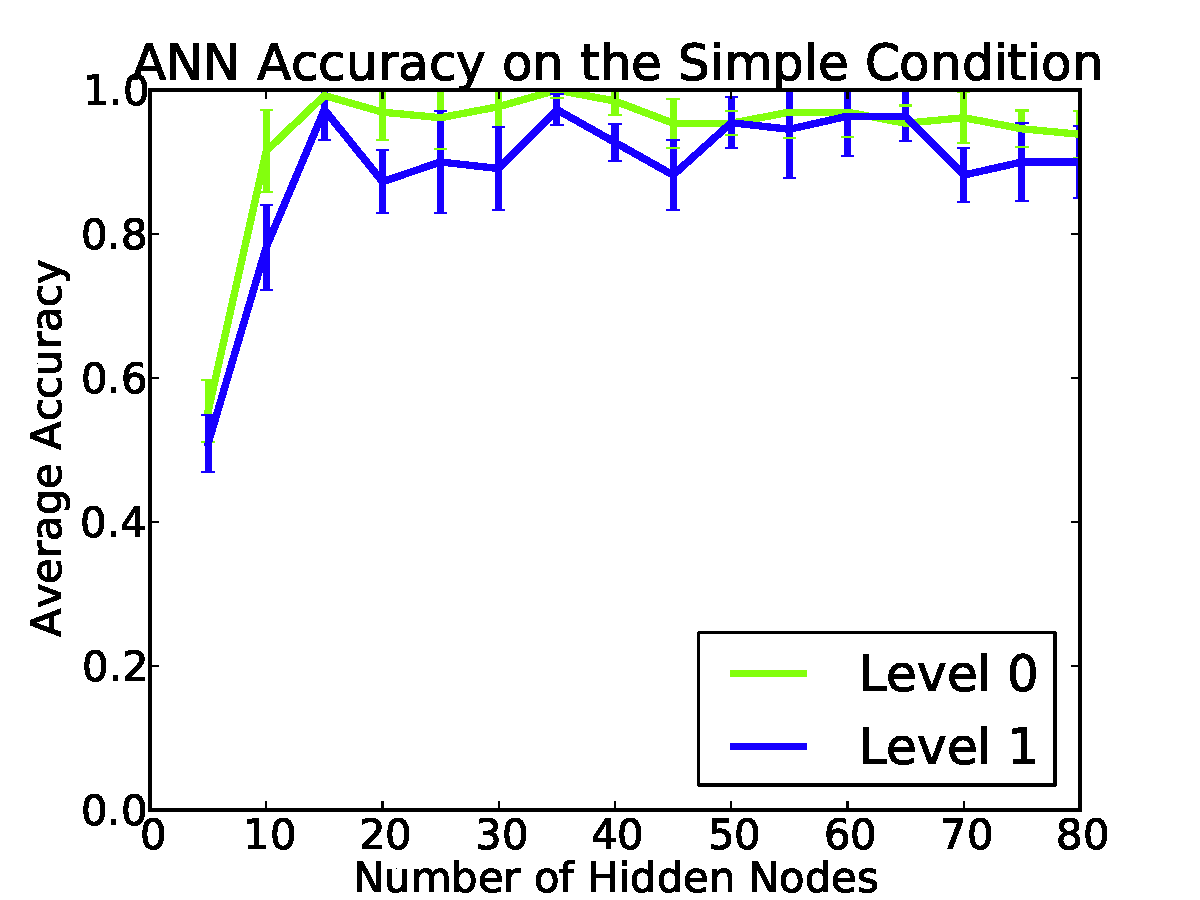
\includegraphics[width=\columnwidth]{fig/hiddenscales.pdf}
%    \caption{\label{fig:hiddenScales}ANN accuracy with a varying number of hidden nodes on the simple condition.}
%\end{figure}
%\begin{figure}
%    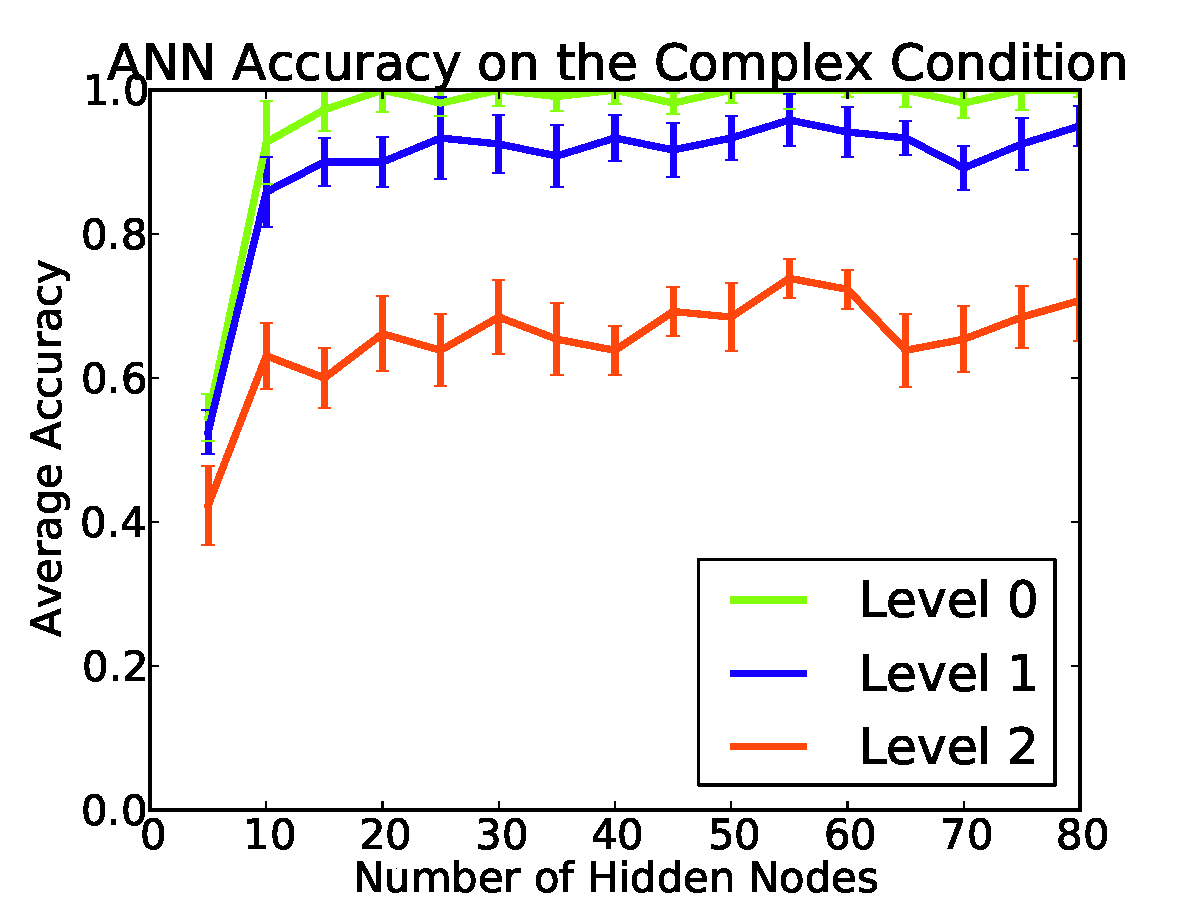
\includegraphics[width=\columnwidth]{fig/hiddenscalesPlus.pdf}
%    \caption{\label{fig:hiddenScalesPlus}ANN accuracy with a varying number of hidden nodes on the complex condition.}
%\end{figure}


\section{Experiment 1: Simple Scalar Implicature}

To quantitatively compare our model with human data, we conducted two
experiments with human participants in which we asked them to play
reference games that varied in their inferential complexity. We then
compare performance of human participants to that of our
discriminative model. Our first experiment used the simple referential
context shown in the left of Figure \ref{fig:humans}, following
\cite{Stiller:Goodman:Frank:2011}.

\subsection{Methods}

\subsubsection{Participants}

We recruited 120 participants on Amazon Mechanical Turk, of whom 65
received the level 0 stimulus, and 55 received the level 1 stimulus.

\subsubsection{Stimuli}

For each participant, we generated a reference game with an underlying
matrix description identical to that shown in the left of
Figure~\ref{fig:humans}. We generated the reference game by choosing a
base item randomly from among six possible options: boat, friend
(shown in Figure~\ref{fig:humans}), pizza, snowman, sundae, and
Christmas tree. Each of the possible items had three features that
were plausible additions to the base item. For example, the friend
item has a hat, glasses, and mustache, while the boat item has a sail,
cabin, and motor. For this experiment, we randomly chose two features,
randomly assigning them to rows in the underlying matrix (ensuring,
e.g., that glasses was not always the target feature), and we randomly
assigned targets to positions in the display (ensuring, e.g., that the
target was not always in the middle).

This reference game supports two possible inference types, which we
refer to as ``level 0'' and ``level 1'', following our usage in the
previous section.  In the case of the display shown in
Figure~\ref{fig:humans}, the message ``hat'' unambiguously refers to
the face with the hat and glasses; since there is no inference
necessary, we call this a ``level 0'' problem. In contrast, the
message ``glasses'' could logically refer to the face with a hat and
glasses, or the face with just a hat. A pragmatic inference is
required to conclude that the message refers to the face
\emph{without} a hat; we refer to this as a ``level 1'' problem.


\subsubsection{Procedure}

Participants saw a webpage that first introduced them to an
interlocutor, ``Bob'', who routinely engaged in some action (e.g.,
visiting his friends for the friend item). They then saw a scene like
that shown in Figure~\ref{fig:humans} and read that ``Bob can only say
one word to communicate with you and he says: [target]'', where
[target] indicates the message relating to the particular condition
they had been randomly assigned to (e.g., ``glasses'' for the level~1
inference in Figure~\ref{fig:humans}).  Participants were instructed
to indicate which item they thought was Bob's target via a
3-alternative forced-choice. Afterwards, they completed a simple check
question (provide the interlocutor's name), which we used to exclude
non-compliant participants.

\subsection{Results}

Human performance is plotted in the bar graph in
Figure~\ref{fig:humans}. The level~0 utterance was trivial, with 95\%
of participants choosing correctly. Participants also made a
substantial portion of implicature-consistent responses (75\%) in the
level~1 condition, replicating \cite{Stiller:Goodman:Frank:2011}.

We next compare human performance to the ANN listener model, which was
trained on $\Gsep$. The accuracy of an ANN listener with 50 hidden
nodes is shown in Figure~\ref{fig:scales}, for a variety of training
iterations. The case of 0 training iterations corresponds to the
literal listener $L_{0}$. We see that the literal listener gets all of
the level~0 (unambiguous) problems correct, and 50\% of the level~1
problems. The ANN slightly outperforms the humans but is well aligned
with them: 91\% accuracy on the level~0 problems, and 86\% accuracy on
the level~1 problems.

%We also explored the effect the size of the hidden layer has on model performance, displayed in Figure \ref{fig:hiddenScales}. Listeners with very limited hidden layers do not learn the task, but do well after using 15 hidden nodes or more.

Lastly, we evaluated the iterated best response (IBR) model on this
condition, shown in Figure~\ref{fig:ibrScales}. The IBR model is
always correct on the level 0 problems, and quickly increases in
accuracy on the level 1 problems as the depth of recursion
increases. This evaluation uses the IBR probabilities to compute
accuracy. If we instead evaluate by predicting the target with highest
probability for each message, it gets all of the level 1 problems
correct after one level of recursion.


\section{Experiment 2: Complex Scalar Implicature}

\subsection{Methods}

\subsubsection{Participants} 

We recruited 180 participants from Mechanical Turk, with 55 receiving
the level 0 stimulus, 60 receiving level 1, and 65 receiving level 2.

\subsubsection{Stimuli}

Stimuli were generated identically to those in Experiment~1, except
that we used the base matrix shown on the right in
Figure~\ref{fig:humans}. With the setting shown there, the message
``hat'' is level~0, ``mustache'' is level~1, and ``glasses'' is
level~2.

\subsubsection{Procedure}

The procedure was identical to Experiment 1. 

\subsection{Results}

Figure~\ref{fig:humans} shows human performance on the more complex
scalar implicature task. Similar to the simple task, 95\% correctly
identified the level~0 referent, and 77\% correctly picked the level~1
referent. However, humans had much more trouble with the level~2
inference, with just 52\% selecting the correct referent given the
utterance.

These results too align with the ANN model
(Figure~\ref{fig:scalesPlus}). We see similar performance on the
level~0 and level~1 problems as in the previous
experiment. Importantly, the model also has much more difficulty with
the level~2 problems (70\% accuracy), which persists across number of training
iterations. Although the model is more accurate than the human
subjects, the results are qualitatively similar. 

This stands in marked contrast to the IBR model's performance, summarized in
Figure~\ref{fig:ibrScalesPlus}. This model always gets the level~0
problems correct. As the depth of recursion increases, the IBR
confidence asymptotes to 1. In the same way as in the simple
condition, if we instead evaluate the IBR model by choosing the
highest probability target for each message, it correctly identifies
the level~1 targets after one step of recursion, and all of the
level~2 problems after two steps of recursion, thereby vastly
outperforming our human subjects.


\section{Conclusion}
We presented a discriminative model of communication that embodies the
central insights of recursive generative models of pragmatic reasoning
but is more computationally efficient, particularly at decision
time. Using experiments involving simple and complex reference games,
we showed that the model displays human-like pragmatic behavior.  In
closing, we note that the models have additional advantages that we
were unable to explore here, including (i) the ability to reason in
terms of partial, heterogeneous representations of the environment,
(ii) a decoupling of inferential power (depth of iteration) from
memory (dimensionality of the hidden representations), and (iii) a
level of computational efficiency that makes them scalable to truly 
massive problems involving language and action together.



\bibliographystyle{apacite}
\setlength{\bibleftmargin}{.125in}
\setlength{\bibindent}{-\bibleftmargin}
\bibliography{ann-ibr}
\end{document}
